\documentclass[a4paper,10pt]{article}

\usepackage[T1]{fontenc}
\usepackage[utf8]{inputenc}
\usepackage[top=0.8cm,bottom=0.8cm,left=1.0cm,right=1.0cm]{geometry}
\usepackage{titlesec}
\usepackage{enumitem}
\usepackage{hyperref}
\usepackage{xcolor}
\usepackage{graphicx}

\definecolor{accent}{HTML}{1F4E78}
\hypersetup{colorlinks=true, urlcolor=accent, linkcolor=accent}
\pagestyle{empty}
\setlength{\parindent}{0pt}

\titleformat{\section}{\large\bfseries\color{accent}}{}{0em}{}[\vspace{-0.6em}\rule{\textwidth}{0.8pt}]
\titlespacing{\section}{0pt}{2pt}{1pt}

\newcommand{\role}[4]{%
 \textbf{#1} \hfill \textbf{#2}\\[1pt]%
 \textit{#3} \hfill \textit{#4}\\[2pt]%
}
\setlist[itemize]{leftmargin=1.2em, itemsep=0pt, topsep=1pt, parsep=0pt}

\begin{document}

% ================= HEADER =================
\begin{minipage}[c]{0.80\textwidth}
 {\Huge\bfseries Prabhavit Gupta}\\[3pt]
 {\color{accent}\large Computerized System Validation (CSV) \& Automation Engineer -- GAMP 5, System Qualification \& Integration}\\[6pt]
 {\footnotesize +39 351 610 7807 ~$\vert$~
 \href{mailto:prabhavitg@gmail.com}{prabhavitg@gmail.com} ~$\vert$~
 \href{https://www.linkedin.com/in/prabhavit/}{linkedin.com/in/prabhavit} ~$\vert$~
 \href{https://github.com/prab-gupta}{github.com/prab-gupta} ~$\vert$~
 Venice, Italy}
\end{minipage}\hfill
\begin{minipage}[c]{0.18\textwidth}
 \raggedleft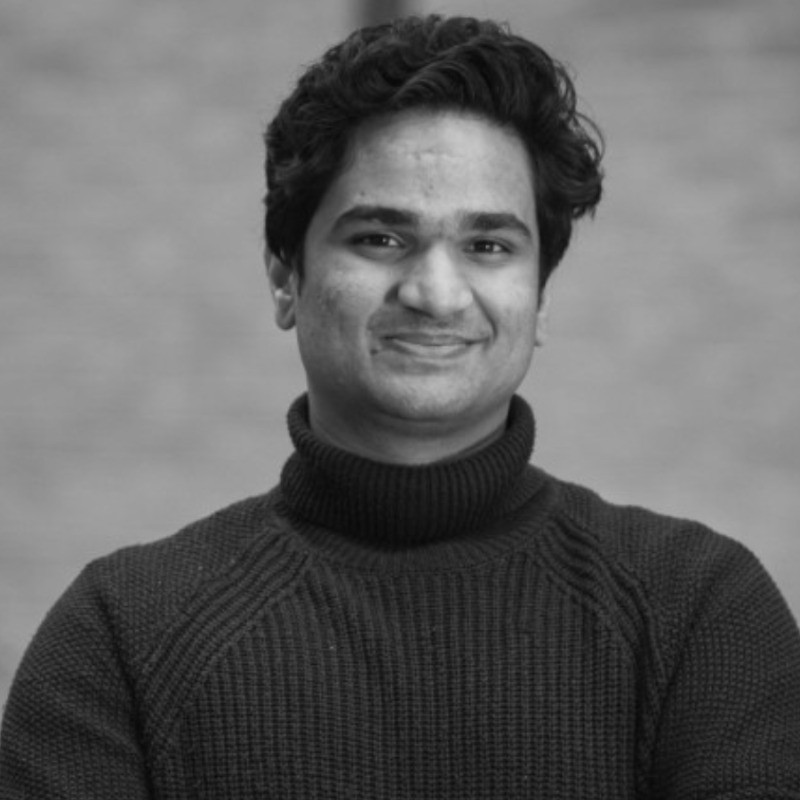
\includegraphics[width=2.0cm]{photo.jpg}
\end{minipage}
\vspace{-2pt}

% ================= SUMMARY =================
\section{Summary}
Systems and Validation Engineer specialized in Computerized System Validation (CSV), data integrity compliance, and automated process qualification. At FlowSpace I established structured validation and testing protocols for production data pipelines and multi-system integrations: I drafted technical requirement specifications (URS), test scripts, and change control procedures adhering to rigorous data governance and auditability standards. I managed end-to-end API integrations and analytics reporting platforms (OfficeRnD, Nexudus, Stripe), executed qualification runs, and resolved deviations through root-cause analysis. Experienced in cross-functional collaboration with QA, software vendors, and operations teams to sustain systems in a verified, compliant state. Based in Italy, European Long Term Residence Permit, available immediately.

% ================= SKILLS =================
\section{Skills}
\begin{itemize}
 \item \textbf{CSV \& Quality Assurance:} Computerized System Validation (CSV), GAMP 5 principles, FDA 21 CFR Part 11, Data Integrity (ALCOA+), URS, Risk Assessments, IQ/OQ/PQ protocols, Change Control, Deviation/CAPA management
 \item \textbf{Automation \& Systems Integration:} Automated workflow orchestration, n8n, Microsoft Power Automate, Tray.ai, REST/GraphQL APIs, OAuth2, Webhooks, custom connectors, MES/ERP integration concepts
 \item \textbf{Data Management \& Analytics:} PostgreSQL, MySQL, Supabase, database schema validation, data migration, Power BI / reporting dashboards, audit trail logging
 \item \textbf{Technical \& Infrastructure:} Python, TypeScript, React, Next.js, Node.js, Docker, Linux, Git, technical SOP authoring, vendor management
\end{itemize}

% ================= EXPERIENCE =================
\section{Experience}

\role{\href{https://flowspace.co}{FlowSpace.co}}{Mar 2024 -- Aug 2026}{Full-Stack \& AI Engineer (Full-time, Freelance)}{London, UK (remote)}
\begin{itemize}
 \item Integrated OfficeRnD and Nexudus APIs end to end: connect flow, location sync, resource mapping, and automated bookings. Owned the full integration lifecycle from technical scoping to production.
 \item Ran technical onboarding for new workspace providers joining the platform. Configured their accounts, mapped their data, and resolved issues directly.
 \item Built an AI listing bot: takes a brochure in any format (PDF, web, photo, spreadsheet), drafts the listing via LLM, routes through human review, then pushes to the backend.
 \item Migrated the platform off a legacy stack to Next.js and Laravel. Mapped the data model, drove the cutover while the product stayed live. Scaled from 2,000 to 4,500+ users.
 \item Built CRM and GTM automations with n8n, plus AI support agents that answer queries against live platform data.
\end{itemize}

\role{\href{https://get2germany.com}{Get2Germany.com}}{Jan 2024 -- May 2024}{Developer \& Automation Specialist (Part-time)}{Berlin, Germany}
Integrated Google APIs, built AI tools to find courses, internships and jobs, and optimized the database. Stack: n8n, Google APIs.\\[1pt]

\role{\href{https://clubee.com}{Clubee.com}}{Sep 2023 -- Aug 2024}{Developer \& QA (Full-time, Freelance)}{Foetz, Luxembourg}
Integrated the Clubee API across the frontend, ran unit testing and QA, and built shop and federation-dashboard tools.\\[1pt]

\role{\href{https://tractionboard.co}{Tractionboard.co}}{Aug 2023 -- Oct 2023}{Developer (Internship)}{Utrecht, Netherlands}
Integrated ChatGPT/OpenAI and Sendgrid, built responsive designs, and debugged features.

% ================= FREELANCE PROJECTS =================
\section{Freelance Projects}
\begin{itemize}
 \item \textbf{\href{https://smarturlink.com/}{Urlink}} (2025), Project Manager \& AI-Assisted Developer. Worked directly with the client on requirements, built the platform and its logic, and implemented client-driven automations. Stack: Next.js, Supabase, Netlify.
 \item \textbf{\href{https://ultrastrategy.com}{UltraStrategy}} (2024 to 2025), AI Automation Developer. Built a CV-parsing tool (LLM data extraction) with n8n and Eden AI, and a platform serving different user profiles.
 \item \textbf{\href{https://www.qomodo.me/}{Qomodo}} (2024 to 2025), AI Developer. Built a branch-management dashboard for companies, and implemented Figma designs.
\end{itemize}

% ================= CERTIFICATIONS =================
\section{Certifications}
Microsoft Copilot Studio Agent Academy \textbullet\ Microsoft: Introduction to building AI agents \textbullet\ Microsoft Power Automate \textbullet\ Tray.AI Build Practitioner (Sep 2024)

% ================= EDUCATION =================
\section{Education}
\textbf{Ca' Foscari University of Venice} \hfill Oct 2020 -- Jun 2024\\
BA Philosophy, International Studies \& Economics (Minor: Entrepreneurship)

% ================= AUTH =================
\vspace{2pt}
{\small \textbf{Work authorization:} European Long Term Residence Permit (Italy), no sponsorship needed in the EU; available immediately. \quad \textbf{Languages:} Hindi (native), English (professional), Italian (beginner).}

\end{document}
